\documentclass{article}
\usepackage[francais]{babel}
\usepackage[T1]{fontenc}
\usepackage[utf8]{inputenc}
\usepackage{lipsum}
\usepackage{pifont}
\usepackage{graphicx}

% mise en page
\usepackage[left=3cm, right=3cm, top=1.5cm, bottom=1.5cm]{geometry}
\usepackage{fancyhdr}

\title{exercice : serie 4}
\author{tom.rsr }
\date{January 2019}

\begin{document}

\maketitle

\section{Avant propos}
Pour effectuer les exercices de cette feuille, vous devrez inclure les paquets$^1$:

\begin{description}
\item[ --- lipsum : ] faux texte de remplissage
\item[ --- pifont : ] caractères spéciaux
\item[ --- graphicx : ] insertion d'images
\end{description}
 
\section{Les paragraphes}

\subsection{Justification}
 Le faux texte ci-dessous est constitué de paragraphes du paquet lipsum

\subsubsection{Texte justifié}
\lipsum[1]

\subsubsection{Texte aligné à droite}
\begin{flushright} 
    \lipsum[2]
\end{flushright}
\subsubsection{Texte aligné à gauche}
\begin{flushleft}
    \lipsum[3]
\end{flushleft}
\subsubsection{Texte centré}
\begin{center}
    \lipsum[4]
\end{center}

\subsection{Espaces verticaux entre les paragraphes}
Placez un espace de 2,3 cm (exactement entre les 2 paragraphes suivants)
\vspace{5mm}
\lipsum[5]
\vspace{2,3cm}
\lipsum[6]
\section{Listes}
\subsection{Listes numérotées}
Classes de documents :
\begin{enumerate}
    \item book
    \item report
    \item article
    \item letter
  \end{enumerate}
\subsection{Listes non numérotées (avec puces)}
\begin{itemize}
    \item book
    \item report
    \item article
    \item letter
  \end{itemize}
\subsection{Listes non numérotée (avec puces modifiées)}
\begin{itemize}
    \item[$\clubsuit $] book
    \item[$\Sigma $] report
    \item[Texte libre] article
    \item[\ding{36}] letter 
\end{itemize}
\section{insertion d'images}
Le fichier cigales\_fourmi.jpg se trouve sur le réseau.
\subsection{Image centrée}
Largeur de l'image = 3,5 cm
\begin{figure}[h]
    \centering
    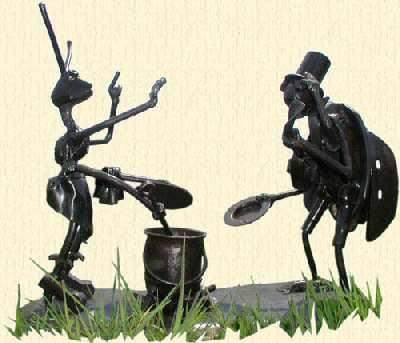
\includegraphics[width=3.5cm]{images/cigale_fourmi.jpg}
    \caption{\label{étiquette} titre}
 \end{figure}
\end{document}
